\documentclass[12pt,a4paper]{article}
%%%! Tjulin: I would use \documentclass[12pt,a4paper]{article} for the benefit of European printers 
%% JW: DONE

% \usepackage{array}
% \usepackage{pbox}
% \usepackage{hanging}
\usepackage{fancyhdr}
% \usepackage{caption}
% \usepackage{enumitem}
\usepackage{fancyvrb}
\usepackage{color}
\usepackage{xcolor}
\usepackage[utf8]{inputenc}
\usepackage{graphicx}
\usepackage{listings}
\usepackage{url}
\usepackage[titletoc,title]{appendix} %%%! Tjulin: Added this for the appendices. 
%% JW Thanks.

\usepackage{xspace}

\usepackage{rotating}
\usepackage{wrapfig}
\usepackage{hyperref}

\usepackage{cite} %

\usepackage[gen]{eurosym}

% \usepackage{todonotes}
\usepackage[colorinlistoftodos,prependcaption,textsize=small]{todonotes}
\newcommand{\tobedone}[2][1=]{\todo[inline,linecolor=red,backgroundcolor=red!25,bordercolor=red]{#2}}
%% \renewcommand{\todo}[1]{\textcolor{red}{TODO: #1}}

\usepackage{draftwatermark}
\SetWatermarkText{draft}
\SetWatermarkScale{6}

\fancypagestyle{plain}{ %
  \fancyhf{} % remove everything
  \renewcommand{\headrulewidth}{0pt} % remove lines as well
  \renewcommand{\footrulewidth}{0pt}
}

\hyphenation{EISCAT}

\newenvironment{MYitemize}{%
    %% \renewcommand{\labelitemi}{$\rightarrow$}%
    %% \renewcommand{\labelitemii}{$\circ$}%
    %% \renewcommand{\labelitemii}{$\rightarrow$}%
    %% \renewcommand{\labelitemiii}{$\rightarrow$}%
    %% \renewcommand{\labelitemiii}{\colblack $\cdot$}%
    \begin{itemize}}{\end{itemize}}

\newcommand{\bitm}{\begin{MYitemize}}
\newcommand{\eitm}{\end{MYitemize}}

\newcommand{\ED}{EISCAT\_3D\xspace}
\newcommand{\EC}{EISCAT\xspace}
\newcommand{\ESA}{EISCAT Scientific Association\xspace}
\newcommand{\SA}{sub-array\xspace}
\newcommand{\SAs}{sub-arrays\xspace}
\newcommand{\RS}{radar site\xspace}
\newcommand{\RSs}{radar sites\xspace}
\newcommand{\OS}{on-site\xspace}
\newcommand{\OC}{operations centre\xspace}
\newcommand{\CC}{control centre\xspace}
\newcommand{\DC}{data centre\xspace}
\newcommand{\DCs}{data centres\xspace}
\newcommand{\UAF}{User Analysis Facility\xspace}

\newcommand{\RB}{ring buffer\xspace}
\newcommand{\fsru}{first stage receive unit\xspace}
\newcommand{\FW}{file writer\xspace}
\newcommand{\SBF}{second beam former\xspace}

\newcommand{\NBW}{5~MHz} % narrow bandwidth
\newcommand{\WBW}{30~MHz} % wide bandwidth

\newcommand{\ramf}{Ramfjordmoen\xspace}
\newcommand{\controllatency}{less than $5$\xspace}
\newcommand{\HDF}{HDF5\xspace}
\newcommand{\einfra}{e-infrastructure\xspace}
\newcommand{\einfras}{\einfra{s}\xspace}
\newcommand{\WR}{White Rabbit\xspace}
\newcommand{\UAP}{User access portal\xspace}

\newcommand{\bfmust}{\xspace{\bf must}\xspace}
\newcommand{\bfshould}{\xspace{\bf should}\xspace}
\newcommand{\Bfmust}{\xspace{\bf Must}\xspace}
\newcommand{\Bfshould}{\xspace{\bf Should}\xspace}
\newcommand{\bfshall}{\xspace{\bf shall}\xspace}
\newcommand{\Bfshall}{\xspace{\bf Shall}\xspace}

\newcommand{\FirstBF}{\xspace{\bf Shall}\xspace}

\newcommand{\visroot}{isualiz}
\newcommand{\vis}{\visroot{ation}\xspace}
\newcommand{\vise}{\visroot{e}\xspace}
% \newcommand{\Vis}{{Visualization}\xspace}
\newcommand{\threed}{{3-dimensional}\xspace}
\newcommand{\GD}{{GUISDAP}\xspace}

\newcommand{\gps}{{Gbit/s}\xspace}


\newcommand\EatDot[1]{}



% \setlength{\topskip}{0mm}
\setlength{\headheight}{15pt}
% \setlength{\topmargin}{-5.4mm}
% \setlength{\textheight}{230mm}
\setlength{\textwidth}{180mm}
\setlength{\oddsidemargin}{-5.0mm}
% \setlength{\evensidemargin}{10.0mm}
% \setlength{\captionmargin}{7mm}

\title{
{\bf \ED Wide Area Network options} \\
E3DDS note on options for online computing}
\author{E3DDS Team~\footnote{
Anders Tjulin (EISCAT) {\tt anders.tjulin@eiscat.se};
Ari Lukkarinen (CSC) {\tt ari.lukkarinen@csc.fi};
Assar Westman (EISCAT) {\tt Assar.Westman@eiscat.se};
Carl-Fredrik Enell (EISCAT) {\tt carl-fredrik.enell@eiscat.se};
Dan Johan Jonsson (UiT) {\tt dan.jonsson@uit.no};
Janos Nagy (NSC) {\tt fconagy@nsc.liu.se};
Harri Hellgren (EISCAT) {\tt harri@eiscat.se};
Ingemar H\"{a}ggstr\"{o}m (EISCAT) {\tt ingemar.haggstrom@eiscat.se};
Mattias Wadenstein (UmU) {\tt maswan@hpc2n.umu.se};
Roy Dragseth (UiT) {\tt roy.dragseth@uit.no};
John White (NeIC) {\tt john.white@cern.ch}}}

\date{\today}

\begin{document}

\pagestyle{fancy}
\lhead{\bf E3DDS project}
\rhead{\bf 1: Hardware and software}

\maketitle
\par\noindent
\begin{minipage}{0.45\textwidth}
  
\includegraphics[scale=0.18]{NEIC_logo_screen_black.pdf}
  %\vspace{-0.09in}
\end{minipage}
\begin{minipage}{0.45\textwidth}
  \hfill
  %
\includegraphics[scale=0.25]{EISCAT3Dlogo1.pdf}
  % New official logo with green text
  
\includegraphics[width=0.75\linewidth]{e3d-logo-green-500px}
\end{minipage}

\begin{center}
\begin{tabular}{|l|l|} \hline
\large \bf Date & \large \bf Comments \\ \hline
\large 2019/11/13 & First draft started \\ \hline
\end{tabular}
\end{center}

\newpage
\tableofcontents
\newpage

\section{Wide-Area Network options considerations}
\label{sec:wan-options}

The \ED sites need to be connected over a Wide-Area Network (WAN).
The WAN must meet capacity and latency requirements to transmit the data produced at the \ED sites, control updates, as well as general remote management, connectivity to the long-term data center storage and direct or indirect connectivity to the internet for users.

The requirement for \ED operations is that the data for \NBW\ case is processed in real-time from antennas to data storage.

\subsection{First Stage Receive Units}
\label{ssec:fsru}
The analogue antenna are converted in an ADC as shown in Figure~\ref{overall}.
One First Stage Receive Unit (FSRU) is attached to each 91~antenna sub-array (109 per site).
The FSRUs take the digitized antenna signals and sample at bandwidths of either \NBW\ or \WBW\ and perform the first stage beam-forming to produce wide-angle beams.

Each FSRU is equipped with two 25~Gb/s ethernet output ports that send the wide-angle beam data, as a UDP stream, to the ring buffer memory.
The data rates per FSRU and per site is shown for the \NBW\ and \WBW\ cases in Table~\ref{tab:fsru-rates-all}.
If the FSRUs are to be upgraded through software or hardware to produce more wide-angle beams then the hard limit for the UDP data stream from a site is: 
25~Gb/s $\times$ 2 $\times$ 109~FSRU = 5.45~Tb/s
.
\begin{table}[h!]
\centering
\begin{tabular}{ccrll|r}
{Bandwidth} & {Beams} & {Bits $\times$}    & Rate    & Sub- & {Total rate} \\
{(digital samples)} & {/FSRU} & {Polarities}       & {/FSRU} & arrays & from site \hfill \\ \hline
& \multicolumn{5}{l}{\bf TX site \NBW\ operations} \\
{\hfill \NBW{} (6.5~MSPS)}& 2 & (16+16)$\times$2 & 830~Mb/s & 119 & 99~Gb/s \\
& \multicolumn{5}{l}{\bf TX site \WBW\ operations} \\
\WBW{} (52~MSPS)& 2 & (16+16)$\times$2 & {\hfill 6.66~Gb/s} & 119 & 792~Gb/s \\
& \multicolumn{5}{l}{\bf RX site \NBW\ operations} \\
{\hfill \NBW{} (6.5~MSPS)} & 10 & (16+16)$\times$2 & 4.16~Gb/s & 109 & 450~Gb/s \\
% \WBW{} (52 MSPS) & 2 & (16+16)$\times$2 & 6.66~Gb/s & 109 & 730~Gb/s \\
& \multicolumn{5}{l}{\bf RX site \WBW\ operations} \\
{\hfill \NBW{} (6.5~MSPS)} & 8 & (16+16)$\times$2 & 3.33~Gb/s & 109 & 363~Gb/s \\
\WBW{} (52 MSPS) & 2 & (16+16)$\times$2 & 6.66~Gb/s & 109 & 726~Gb/s \\
& \multicolumn{5}{l}{\bf Maximum rate \WBW} \\
\WBW{} (52 MSPS) & 10 & (16+16)$\times$2 & 33.3~Gb/s & 109 & 3.63~Tb/s \\
\end{tabular}
\caption{Data rates at \ED sites per FSRU and for whole site to the Ring Buffer memory. The \WBW\ maximum rate mode is not expected to be required by \ED.
\label{tab:fsru-rates-all}}
\end{table}
\iffalse
\begin{table}[h!]
\centering
\begin{tabular}{cccrll|r}
{Site } & {Bandwidth} & {Beams} & {Bits $\times$}    & Rate    & Sub- & {Total rate} \\
& {(digital samples)} & {/FSRU} & {Polarities}       & {/FSRU} & arrays & from site \hfill \\ \hline
{TX} & {\hfill \NBW{} (6.5~MSPS)}& 2 & (16+16)$\times$2 & 830~Mb/s & 119 & 99~Gb/s \\
TX & \WBW{} (52~MSPS)& 2 & (16+16)$\times$2 & {\hfill 6.66~Gb/s} & 119 & 792~Gb/s \\
RX & {\hfill \NBW{} (6.5~MSPS)} & 10 & (16+16)$\times$2 & 4.16~Gb/s & 109 & 450~Gb/s \\
RX & {\hfill \NBW{} (6.5~MSPS)} & 8 & (16+16)$\times$2 & 3.33~Gb/s & 109 & 363~Gb/s \\
 & \WBW{} (52 MSPS) & 2 & (16+16)$\times$2 & 6.66~Gb/s & 109 & 726~Gb/s \\
 & & \multicolumn{5}{l}{\bf Maximum rate \WBW} \\
 & \WBW{} (52 MSPS) & 10 & (16+16)$\times$2 & 33.3~Gb/s & 109 & 3.63~Tb/s \\
\end{tabular}
\caption{Data rates at \ED sites per FSRU and for whole site to the Ring Buffer memory.
\label{tab:fsru-rates-all}}
\end{table}
\fi
\subsubsection{Skibotn site}
The Skibotn site is both transmitter (TX) and receiver (RX) so the number of any wide angle beams is reduced.
In both the \NBW\ and \WBW\ operations 2 wide-angle beams are produced.

Table~\ref{tab:fsru-rates-all} gives the total data rate from all sub-array first beam-formers at the Skibotn TX/RX site.
For the \NBW{} ``continuous" operation there will be~2 wide-angle beams per FSRU,  each FSRU will transmit 830 Mb/s.
The the total data rate from all sub-arrays to the ring buffer memory in \NBW{} bandwidth will be~99~Gb/s.

For the \WBW{} bandwidth mode, anticipated to run only in a ``burst" mode, there are 2~beams per~FSRU over all the 119~sub-arrays as, by definition, the radar TX and RX directions are along the same line of site at the TX station.
As the \NBW{} and \WBW{} bandwidths are operated simultaneously, the  total data rate is summed to produce 891~Gb/s.
\iffalse \begin{table}[h]
\centering
\begin{tabular}{ccrlr|r}
{Bandwdith} & {Beams} & {Bits $\times$}    & Rate    & Sub- & {Total rate} \\
{(digital samples)} & {/FSRU} & {Polarities} & {/FSRU} & arrays & \\ \hline
{\hfill \NBW{} (6.5~MSPS)}& 2 & (16+16)$\times$2 & 830~Mb/s & 119 & 99~Gb/s \\
\WBW{} (52~MSPS)& 2 & (16+16)$\times$2 & {\hfill 6.66~Gb/s} & 119 & 792~Gb/s \\
\end{tabular}
\caption{Data rates at the TX/RX site per FSRU and for whole site to online data processing nodes for the \NBW\ and \WBW\ cases.. \label{tab:skib:rates}}
\end{table} \fi
\subsubsection{Receive sites}

The Receive (RX) sites are distant ($\approx 200$~km) to the transmitter and therefore the maximum number (10) of wide-angle beams are produced.
%% in order to mantain resolution (check technical description).
Table~\ref{tab:fsru-rates-all} gives the total data rate from all sub-array first beam-formers at the RX sites.
\iffalse \begin{table}[h!]
\centering
\begin{tabular}{ccrll|r}
{Bandwidth} & {Beams} & {Bits $\times$}    & Rate    & Sub- & {Total rate} \\
{(digital samples)} & {/FSRU} & {Polarities}       & {/FSRU} & arrays & \\ \hline
{\hfill \NBW{} (6.5~MSPS)} & 10 & (16+16)$\times$2 & 4.16~Gb/s & 109 & 450~Gb/s \\
% \WBW{} (52 MSPS) & 2 & (16+16)$\times$2 & 6.66~Gb/s & 109 & 730~Gb/s \\
\end{tabular}
\caption{Data rates at RX sites per FSRU and for whole site to online data processing nodes for the \NBW\ case. \label{tab:rx:rates}}
\end{table} \fi

\iffalse \begin{table}[h!]
\centering
\begin{tabular}{ccrll|r}
{Bandwidth} & {Beams} & {Bits $\times$}    & Rate    & Sub- & {Total rate} \\
{(digital samples)} & {/FSRU} & {Polarities}       & {/FSRU} & arrays & \\ \hline
{\hfill \NBW{} (6.5~MSPS)} & 8 & (16+16)$\times$2 & 3.33~Gb/s & 109 & 363~Gb/s \\
\WBW{} (52 MSPS) & 2 & (16+16)$\times$2 & 6.66~Gb/s & 109 & 726~Gb/s \\
\end{tabular}
\caption{Data rates at RX sites per FSRU and for whole site to online data processing nodes for the \WBW\ case. \label{tab:rx:rates2}}
\end{table} \fi

In the \NBW{} bandwidth ``continuous" operation there are~10 wide-angle beams per FSRU, each FSRU will transmit 4.2~Gb/s for a total rate to the ring buffer of 450~Gb/s.

In the \WBW{} bandwidth mode, anticipated to run only in a ``burst" mode, the 10 beams total consist of 8~\NBW\ and 2~\WBW~beams per sub-array.
In the \WBW{} bandwidth case, the \WBW{} and \NBW{} rates are summed for a total of 1.09~Tb/s of UDP stream data sent to the ring buffer.

The maximum data rate when producing wide-angle beams is when the FSRUs produce 10~wide-angle beams in \WBW\ mode, as shown in Table~\ref{tab:fsru-rates-all}.
\iffalse \begin{table}[h!]
\centering
\begin{tabular}{ccrll|r}
{Bandwidth} & {Beams} & {Bits $\times$}    & Rate & Sub- & {Total rate} \\
{(digital samples)} & {/FSRU} & {Polarities}       & {/FSRU} & arrays & from site\\ \hline
% {\hfill \NBW{} (6.5~MSPS)} & 8 & (16+16)$\times$2 & 3.33~Gb/s & 109 & 363~Gb/s \\
\WBW{} (52 MSPS) & 10 & (16+16)$\times$2 & 33.3~Gb/s & 109 & 3.63~Tb/s \\
\end{tabular}
\caption{Data rates at RX sites per FSRU and for whole site to online data processing nodes for the \WBW\ case. \label{tab:rx:rate-max}}
\end{table} \fi

\subsection{Second Beam Former}

The Second Beam Former (SBF) reads data in the ring buffer from all sub-arrays and produces 10 narrow angle beams per wide-angle beam.

At the TX site the output rate from the Second Beam Former (SBF) in \NBW\ operation is:
6.5~MSPS $\times$ (32+32)~bits/beam $\times$ 40~beams $\approx$ 17~Gb/s. \\
At each of the RX sites, 6.5~MSPS $\times$ (32+32) bits/beam 
$\times$ 200 beams $\approx$ 83~Gb/s.

At both the TX and RX sites, the output rate from the SBF in \WBW\ operation is: \\
52~MSPS $\times$ (32+32)~bits/beam $\times$ 40~beams $\approx$ 133~Gb/s.
Note that the \WBW\ data is not required to be processed in real time (see Section~\ref{sec:wan-options}).

\iffalse
\begin{table}[h!]
\centering
\begin{tabular}{ccr|r}
{Bandwidth} & {Beams} & {Bits $\times$} & {Total rate} \\
{(digital samples)} &  & {Polarities}  & \\ \hline
\multicolumn{4}{l}{\bf TX site \NBW\ operations} \\
{\hfill \NBW{} (6.5~MSPS)}& 40 & (32+32)$\times$2 & 17~Gb/s \\
\multicolumn{4}{l}{\bf RX site \NBW\ operations} \\
{\hfill \NBW{} (6.5~MSPS)}& 200 & (32+32)$\times$2 & 83~Gb/s \\
\multicolumn{4}{l}{\bf TX/RX site \WBW\ operations} \\
{\hfill \WBW{} (52~MSPS)}& 40 & (32+32)$\times$2 & 133~Gb/s \\
\
\end{tabular}
\caption{Data rates at \ED sites per FSRU and for whole site to the Ring Buffer memory.
\label{tab:sbf-rates-all}}
\end{table}
\fi
\begin{table}[h!]
\centering
\begin{tabular}{lcrr|r}
{Site} & {Bandwidth} & {Beams} & {Bits $\times$} & {Total rate} \\
 & {(digital samples)} &  & {Polarities}  & \\ \hline
% \multicolumn{4}{l}{\bf TX site \NBW\ operations} \\
TX & {\hfill \NBW{} (6.5~MSPS)}& 40 & (32+32)$\times$2 & 17~Gb/s \\
% \multicolumn{4}{l}{\bf RX site \NBW\ operations} \\
RX & {\hfill \NBW{} (6.5~MSPS)}& 200 & (32+32)$\times$2 & 83~Gb/s \\
% \multicolumn{4}{l}{\bf TX/RX site \WBW\ operations} \\
TX/RX & {\hfill \WBW{} (52~MSPS)}& 40 & (32+32)$\times$2 & 133~Gb/s \\
\
\end{tabular}
\caption{Data rates at \ED sites per FSRU and for whole site to the Ring Buffer memory.
\label{tab:sbf-rates-all}}
\end{table}


\subsection{Prompt computing}

Easy: Divide by 10!

\section{WAN configurations}

The Wide Area Network (WAN) connects the \ED sites through a long-dstance fibre optic-based network.
Here, we make an assumption that a site is designated to contain the ``central" computing and radar operations. 
A logical assumption as the transmitter is physically located at the TX site in Skibotn.

\subsection{IP Routed connections}
\begin{figure}[h]
\centering
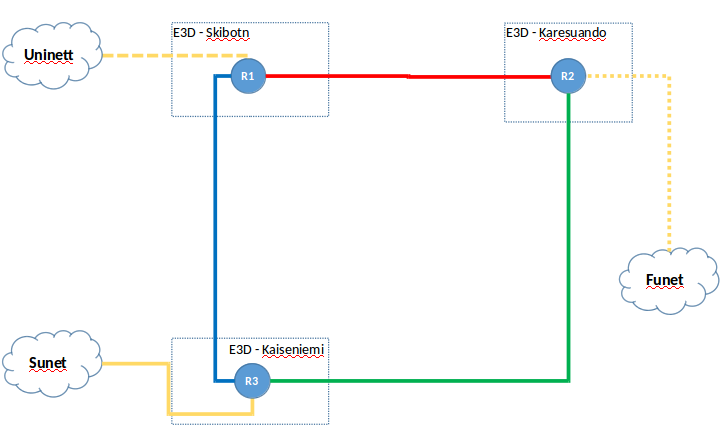
\includegraphics[width=0.7\textwidth]{Site_Connections.png}
\caption{Site connections.\label{fig:site-connections}
}
\end{figure}

Inter-site connectivity is provided by an EISCAT-3D ``LAN'' (IP-routed) ring connecting the local networks of each of the sites.
There is a connection to each National Research and Education Network (NREN) for upstream traffic and the total aggregate ring capacity is 100~Gb/s.
This implies a maximum data rate of 33~Gb/s simultaneous output from each site.

This WAN option requires that the first and second beam forming are performed at each site.
Depending on the output rate of the prompt computing processing, this could be situated at a centralized location on the IP-routed ring.

\subsection{Optical connections}
\label{ssec:optical}

The Dense Wavelength Division Multiplexing~\cite{dwdm} (DWDM), an optical technology used to increase bandwidth over existing fiber optic backbones, provides an attractive alternative for connecting the \ED sites.

DWDM works by combining and transmitting multiple signals simultaneously at different wavelengths on the same fiber. 
In effect, one fiber is transformed into multiple virtual fibers. 
A key advantage to DWDM is that it is protocol and bit-rate independent. 
DWDM-based networks can transmit data in IP and other protocols and can handle bit rates between 100~Mb/s and 2.5~Gb/s. 
Therefore, DWDM-based networks can carry different types of traffic at different speeds over an optical channel.
From a Quality of Service standpoint, DWDM-based networks create a lower cost way to quickly respond to bandwidth demands and protocol changes.

\subsubsection{DWDM Option 1}
Here DWDM is used to connect the three \ED sites to a central location.
\label{sssec:option1}
\begin{figure}[h]
\centering
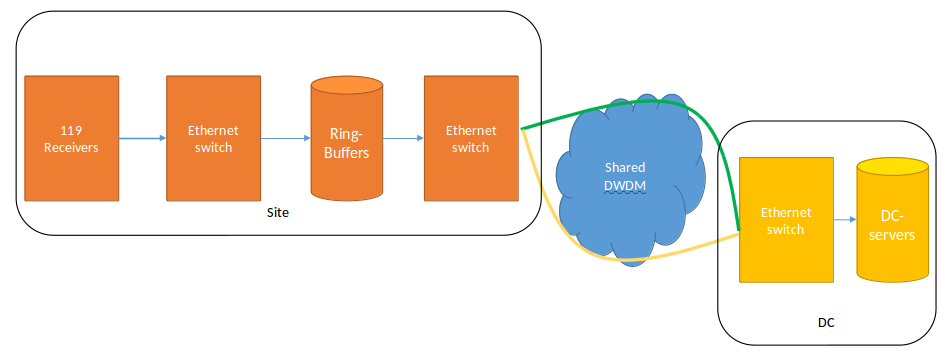
\includegraphics[width=\textwidth]{photon_option_1.png}
\caption{\ED TX/RX sites are connected to a central location via $2\times 100 $~Gb/s DWDM ethernet connections.\label{fig:option_1}
}
\end{figure}
Considering that the requirement is to process \NBW\ online data in realtime.
Working backwards, from prompt computing to FSRUs, along the online data processing chain:
\bitm
\item Prompt computing output can easily be sent over the WAN to central site.
\item The \NBW\ output of the \SBF\ of each RX site (see Table~\ref{tab:fsru-rates-all}) can be sent to a central location for prompt computing processing;
\item The output data rate of the FSRUs, on RX sites in \NBW\ mode, to \RB\ memory is too large (see Table~\ref{tab:sbf-rates-all}) for such a WAN.
\eitm

\subsubsection{DWDM Option 2a}
\label{sssec:option2a}

Here the capacity of the DWDM connection is sized such that the \RB\ nodes are located in the central computing location.
The FSRUs connect to an ethernet switching fabric that subsequently connects to the optical WAN as shown in Figure~\ref{fig:option_2a}.
\begin{figure}[h]
\centering
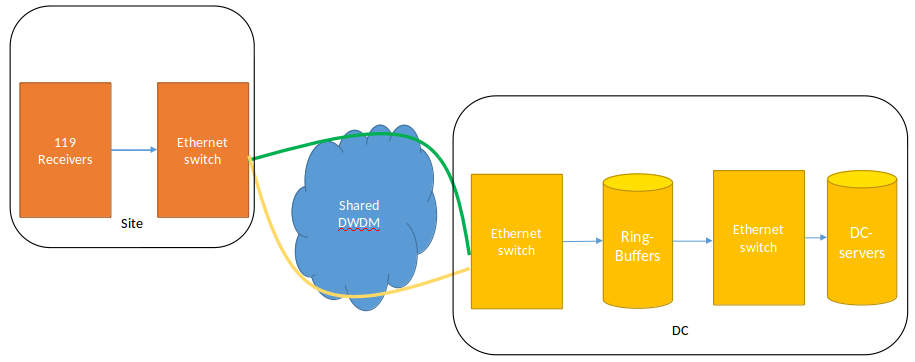
\includegraphics[width=\textwidth]{photon_option_2a.png}
\caption{Site connections.\label{fig:option_2a}
}
\end{figure}
Each DWDM wave has a capacity of 400~Gb/s.
As shown in Section~\ref{}

\subsubsection{Option 2b}
\label{sssec:option2b}
\begin{figure}[h]
\centering
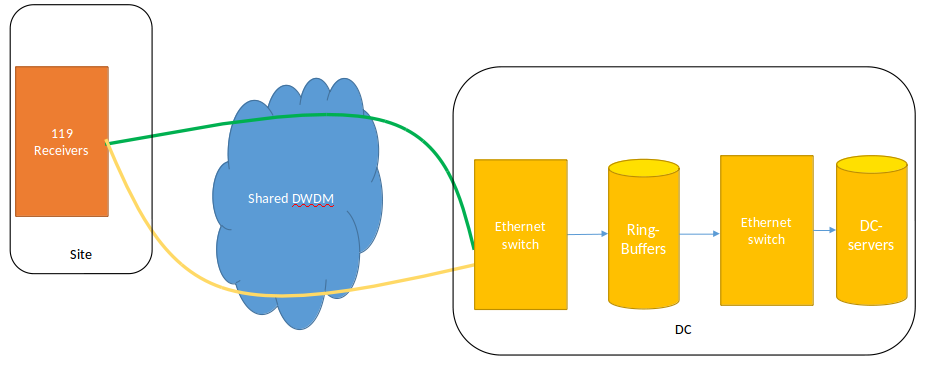
\includegraphics[width=\textwidth]{photon_option_2b.png}
\caption{Site connections.\label{fig:option_2b}
}
\end{figure}

\newpage
\bibliography{main}{}
\bibliographystyle{unsrt}
\end{document}
